\section{Method}
\label{sec:method}

\begin{figure*}[t]
    \centering
    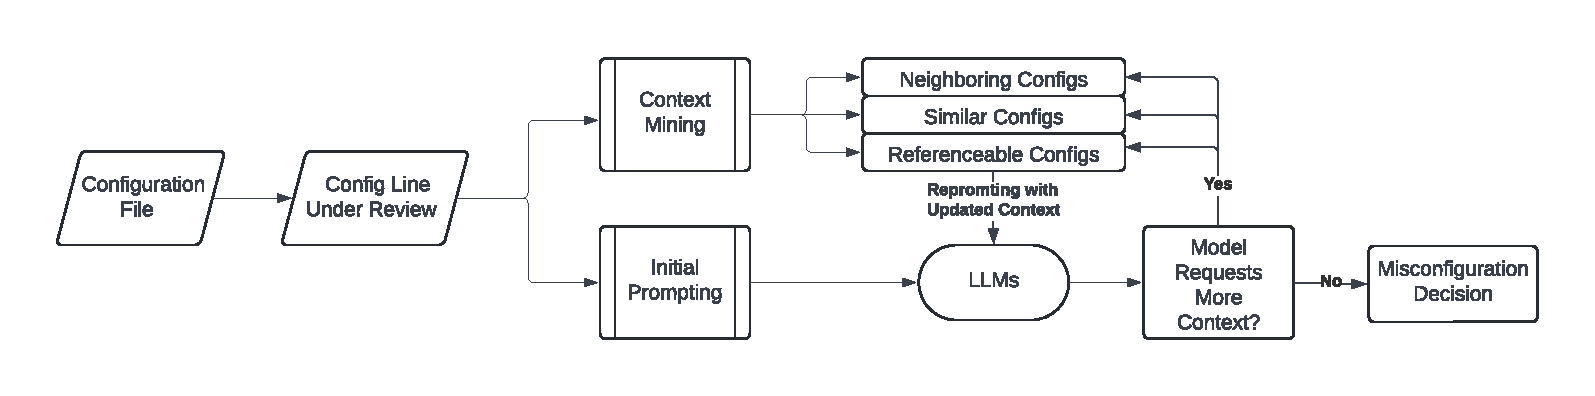
\includegraphics[width=\linewidth]{figs/caip.pdf}
    \caption{\sysname{} system overview.}
    \label{fig:overview}
\end{figure*}

To address the limitations of partition-based prompting, we design \sysname{} (Context-Aware Iterative Prompting), which consists of two core components as shown in Figure~\ref{fig:overview}: an context mining component and an iterative prompting component. These components work together to automate the process of context extraction and prompt interaction with LLMs, enabling more accurate router misconfiguration detection.
\begin{enumerate}
    \item \textbf{Context Mining Component}:
In this phase, \sysname{} automatically mines all relevant context for a given configuration line under examination. Relevance here refers to configurations that, while not necessarily directly related, provide important insights—such as neighboring configurations, similar lines applied in different contexts, or referenceable configurations that define key parameters. This context mining is designed to be both efficient and precise, extracting only the most relevant data from the configuration file without flooding the system with unnecessary information.

    \item \textbf{Iterative Prompting Component}:
Once the relevant context has been mined, the online component engages the LLM through an iterative prompting process. Instead of overwhelming the model with all the extracted context at once, \sysname{} interacts with the LLM in a guided, sequential manner.
\end{enumerate}

We detail the challenges encountered in designing these two components and present the solutions that enable \sysname{} to perform effective context extraction and interactive prompting for misconfiguration detection.
\subsection{Context Mining}\label{mining_method}
\subsubsection{Challenge 1 - Efficient and accurate context mining}
\label{challenge_1}
Configuration files are often lengthy and complex, consisting of multiple interrelated lines that define various aspects of a system's behavior. When analyzing a specific configuration line, it is crucial to efficiently identify and extract the relevant context to reduce the computational burden on LLMs and minimize the risk of introducing irrelevant information that could degrade the accuracy of misconfiguration detection. This task is challenging because, while these configurations are typically written in a machine and human-readable format, automating the process of context extraction requires a deep understanding of the hierarchical and interconnected nature of the configuration data. For example, in a network configuration, a line that specifies an access control rule might be dependent on prior lines that define network segments or user roles. Without properly extracting and understanding this context, the LLM might misinterpret the rule, leading to false positives or missed misconfigurations.

\mypara{Solution} To address this challenge, we can leverage two key observations:
\begin{figure}[t]
    \centering
    \fbox{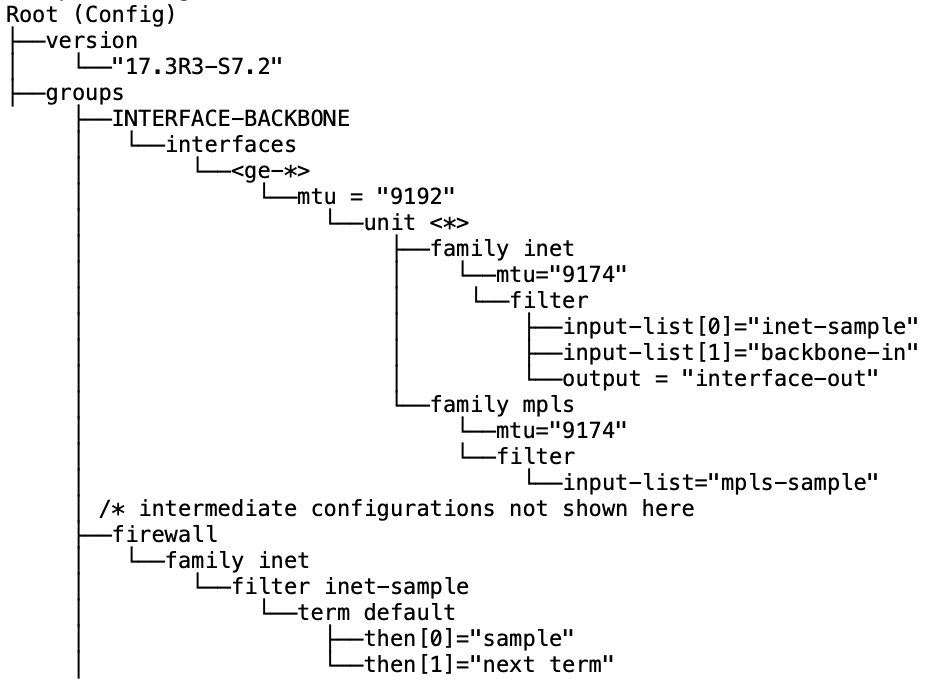
\includegraphics[width=\columnwidth]{figs/tree_form.png}}
    \caption{Example snippet of tree-formatted Junpiter router configuration file.}
    \label{fig:tree}
\end{figure}

\begin{enumerate}
    \item \textit{Hierarchical Structure of Configuration Files}: Configuration files are typically written in a structured, hierarchical format that can be effectively modeled as a tree, as shown in the example in Figure~\ref{fig:tree}. In this tree representation (\(T\)), each node (\(V\)) corresponds to a specific configuration element, and edges represent the relationships or dependencies between these elements. The root node (at level 0) represents the entry point of the configuration file (thus it only serves at the root of the tree and serve no semantic meanings), while the nodes at level 1 (\( L_1 \)) correspond to the broadest configuration categories. Intermediate nodes at subsequent levels (\( L_2, L_3, \dots, L_n \)) represent increasingly nested configuration sections or subcategories, each refining the configuration context. The leaf nodes (or parameter nodes) represent the final configurable parameters, with the associated values (\ie, parameter values) indicating the specific configuration settings. A unique configuration line is thus a complete path in the tree, starting from the root node and terminating at a parameter node, where the path reflects the hierarchical structure and relationships defined in the configuration file.

    \item \textit{Contextual Relevance from Different Aspects}: We make the observation that the context related to any given configuration line can be categorized into three types based on its position and relation within the configuration file as shown in the example in Figure~\ref{fig:context_mine}, with increasing levels of complexity to mine. They each providing unique insights that contribute to accurate misconfiguration detection: 
    \begin{itemize}
        \item \textit{Neighboring Configurations}: Neighboring configurations are those that are closely related to the line under examination, typically within the same section or functional block of the network configuration. For instance, if analyzing a line that defines a VLAN assignment on a particular interface, neighboring configurations would include other lines that configure the same interface or VLAN. These configurations provide insights into how related parameters are set up in proximity, revealing potential dependencies or conflicts. Additionally, by referencing related configurations that define or modify these neighboring parameters, one can understand how changes in one part of the network might impact adjacent configurations, helping to identify misconfigurations that could lead to issues like traffic misrouting or security vulnerabilities. Neighboring configurations are relatively easy to mine because they are identified based on adjacency or location in the configuration file, making them straightforward to extract.
        
        \item \textit{Similar Configurations}: These are configurations that involve the same type of parameter or function as the configuration line under review but are applied in different contexts within the network. For example, consider configurations that assign IP addresses to different interfaces across various routers in the network. Even though the interfaces and routers may differ, the principles governing IP address assignment remain the same. By comparing these similar configurations, one can detect inconsistencies or deviations from standard practices that might indicate a misconfiguration. This type of context is essential for ensuring that configuration practices are consistent across the network, reducing the risk of errors that could lead to network outages or performance degradation. Mining these configurations is more challenging because, unlike neighboring configurations, they are not located adjacently but must be identified based on functional similarities.

        \item \textit{Referenceable Configurations}:
        These configurations provide essential definitions or additional information related to the parameter value being examined. In the network domain, this context is crucial for understanding how specific values are applied across different parts of the network configuration. For example, if a parameter value specifies an import policy, referenceable configurations might include other lines where this policy is defined or where its behavior is modified. By examining these configurations, one can gain a deeper understanding of how the policy influences routing decisions or interacts with other network elements, ensuring that the configuration is applied correctly and consistently throughout the network.
        Referenceable configurations are the most difficult to mine because they often involve indirect references and dependencies that are not immediately apparent, requiring a thorough and sometimes recursive analysis to trace how a value or policy is utilized across various parts of the configuration file.
        \end{itemize}
\end{enumerate}

\begin{figure}[t]
    \centering
    \fbox{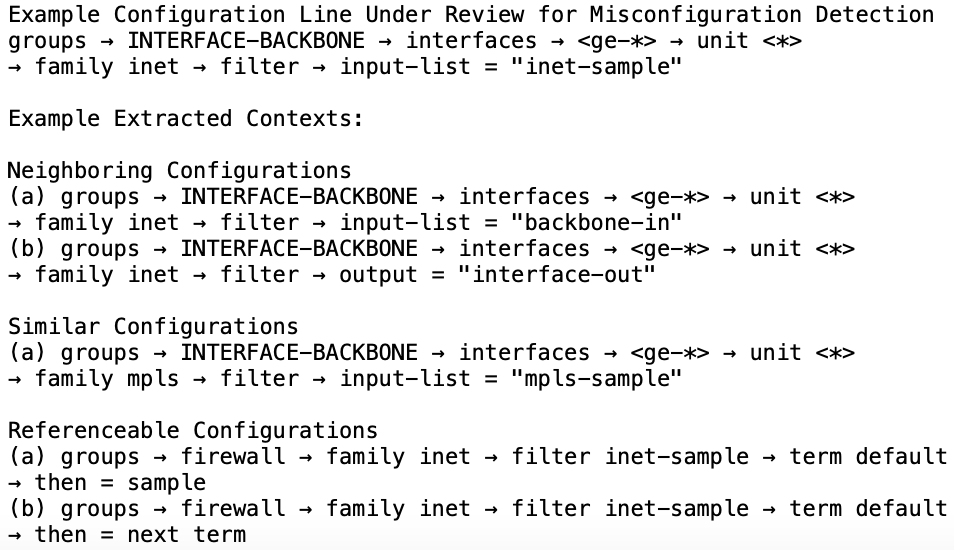
\includegraphics[width=\columnwidth]{figs/context_mine.png}}
    \caption{Example context mined on selected configuration line.}
    \label{fig:context_mine}
\end{figure}

Given the categorization of relevant contexts and the hierarchical tree model, we can automate the process of mining the aforementioned contexts by translating them into specific paths within the tree structure. This involves the following steps:
\paragraph{Neighboring Configuration Mining:}
    Following the hierarchical tree structure of the configuration file, we can model the entire configuration as a tree \( T \) with nodes representing configuration elements and edges depicting the relationships between them. The root node \(V_0\) represents the entry point of the configuration file and the \(L1\) nodes represent the broadest configuration categories.
    For any general configuration path \( P = \{ V_0 \rightarrow A_1 \rightarrow A_2 \rightarrow \dots \rightarrow D = v_D \} \) within the tree, where \(A_1\) is the \(L_1\) node and \( v_D \) is the parameter value assigned to the parameter node \( D \), the goal of neighboring configuration mining is to extract other paths in the tree that share a common sub-path with \( P \) up to a certain depth. 
    
    The common ancestry level, or shared node depth, can be adjusted to control how much context is mined. Let us define \( k \) as the number of shared nodes from the root, then neighboring configurations are defined as:
\[
N_k(P) = \{ P' \in T \mid P' = V_0 \rightarrow \dots \rightarrow V_k \rightarrow V_{k+1} \rightarrow \dots \rightarrow X = v_X \},
\]
where \( P' \) shares the first \( k \) nodes with \( P \), but the nodes following \( V_k \) (denoted as \( V_{k+1}, V_{k+2}, \dots \)) can differ from the remaining nodes in \( P \), and \( X \neq D \) (i.e., \( P' \) does not terminate at \( D \)).

Adjusting \( k \) allows for control over the size and relevance of the neighboring context.
A common choice is to set \( V_k \) as the grandparent node, which captures sufficient context while avoiding unnecessary complexity. For example. let the configuration path under review be represented as:
\[
P = \{V_0 \rightarrow A \rightarrow B \rightarrow C \rightarrow D = v_D \}
\]
Let \( G_P \) represent the grandparent node of \( P \), which in the case of \( P \) would be node \( C \). The set of neighboring paths \( N(P) \) can be defined as:
\[
N(P) = \{ P' \in T \mid P' = V_0 \rightarrow A \rightarrow B \rightarrow C \rightarrow D' = v_{D'}, D' \neq D \}
\]
For example, consider a configuration line that defines the IP address for a particular interface:
\begin{multline*}
P = \{V_0 \rightarrow \text{interfaces} \rightarrow \text{ge-0/0/0} 
\rightarrow \text{unit 0} \rightarrow \text{family inet}\\
\rightarrow \text{address} = 192.168.1.1/24 \}
\end{multline*}
Here, the grandparent node \( G_P \) would be \( \text{`family inet'} \). Neighboring paths in this case might include:
\begin{multline*}
N(P) = \{V_0 \rightarrow \text{interfaces} \rightarrow \text{ge-0/0/0}
\rightarrow \text{unit 0} \rightarrow
\text{family}\\ \text{inet} \rightarrow \text{mtu} = 1500 \}
\end{multline*}
This ensures the extracted neighboring paths are closely relevant, revealing how related parameters are configured in the same section without overwhelming the system with excessive data. Thus, in our evaluation of \sysname{}, we select the grandparent node as  \( V_k \) for an effective balance between relevance and computational efficiency.


\paragraph{Similar Configuration Mining:} To identify similar configurations, we locate paths that share the same entry point root node (\(V_0\)), \(L1\) node (the broadest configuration category), and parameter nodes (\(D\)) but vary in their intermediate nodes or parameter values. Let us again have \(
P = \{ V_0 \rightarrow A \rightarrow B \rightarrow C \rightarrow D = v_D \}
\) to represent a configuration line under review.
Given \( P \), the set of similar configuration paths \( S(P) \) can be defined as:
\[
S(P) = \{ P' : P' = \{ V_0 \rightarrow A \rightarrow X_1 \rightarrow X_2 \rightarrow \dots \rightarrow D = v'_D \} \},
\]
where \( P' \) shares the same \(L1\) node \( A \) and parameter node \( D \), but can have any number of intermediate nodes \( X_1, X_2, \dots \) that differ from the intermediate nodes in \( P \), as well as possibly differing parameter values \( v'_D \).
The reason we use the \( L_1 \) node \( A \) rather than the root node \( V_0 \) is that the \( L_1 \) node represents the broad configuration category or section under which the parameter node \( D \) exists. By focusing on the same \( L_1 \) node, we ensure that we are comparing similar types of configurations within the same category or context, even though the specific paths leading to \( D \) may vary. Using the root node \( V_0 \) would not provide meaningful differentiation, as it encompasses the entire configuration file, making it too general for this analysis. By comparing these variations, we can understand how the same type of parameter is configured, which is essential for ensuring consistency across the network configuration.

For example, let the configuration path under review \( P \) be:
\[
P = \{ V_0 \rightarrow \text{Interfaces} \rightarrow \text{Ethernet0} \rightarrow \text{IP} \rightarrow \text{MTU} = 1500 \}
\]
This represents the configuration for setting the Maximum Transmission Unit (MTU) to 1500 on interface Ethernet0 under the `Interfaces' section.
A similar configuration \( P' \) could be:
\[
P' = \{ V_0 \rightarrow \text{Interfaces} \rightarrow \text{Ethernet1} \rightarrow \text{IP} \rightarrow \text{MTU} = 9000 \}
\]
In this case, \( P' \) shares the same broad configuration category `Interfaces' (\( A \)) and parameter node `MTU' (\( D \)), but differs in the intermediate node `Ethernet1' and the parameter value (9000 vs. 1500). By comparing similar configurations, the context reveals not only the MTU settings but also the intermediate configuration elements leading to the MTU setting across different interfaces within the network configuration.


\paragraph{Referenceable Configuration Mining:} In the hierarchical tree structure, referenceable configurations are identified by locating paths where the parameter node of the current line under review appears as an intermediate node in other paths. This type of context is crucial for understanding how specific parameter values or policies are further referenced, elaborated upon, or applied in other parts of the configuration. we can formalize this  set of referenceable configuration paths \( R(P) \) as:
\[
R(P) = \{ P' : P' = \{ V_0 \rightarrow \dots \rightarrow v_D \rightarrow \dots \rightarrow X \} = v_{X}\}.
\]
In these paths, \( v_D \) is no longer a parameter value, but an intermediate node, meaning it is being referenced or defined further down the configuration hierarchy.

For example, suppose the current configuration line is:
\(V_0 \rightarrow RouterA \rightarrow Policy \rightarrow ImportPolicy = PolicyX\), a referenceable path might be:
\(
V_0 \rightarrow  RouterA \rightarrow Policy \rightarrow PolicyX \rightarrow Filter = AllowAll
\),
indicating that \( PolicyX \) is further applied or modified by the filter configuration. Referenceable configuration mining helps to understand not only how a particular configuration value is defined, but also how it interacts with or influences other components of the network. This process is essential for detecting misconfigurations that arise from improper application or dependency handling across different sections of the configuration file.


% By structuring the context mining process in this manner, we can efficiently and accurately extract the most relevant information for any given configuration line, enhancing the performance and accuracy of LLM-based configuration verification tools. This approach ensures that the LLM receives a well-curated set of contextually relevant data, improving its ability to detect sophisticated misconfigurations that depend on a comprehensive understanding of the configuration file.

However, one of the key problems in extracting referenceable configurations lies in differentiating between \textit{pre-defined} and \textit{user-defined} parameter values. This distinction is crucial because the relevance and interpretation of the mined context depend heavily on whether the parameter value is a built-in element of the configuration language or a custom value defined by the network administrator. We now proceed to discuss this problem in more detail and present our solution.

\subsubsection{Challenge 2 - Referenceable Parameter Value Ambiguity}

In network configurations, parameter values can broadly be categorized into two types: \textit{pre-defined} values and \textit{user-defined} values. Pre-defined values are those that are built into the configuration language itself, such as boolean flags (True vs. False) or access control decisions (Allow vs. Deny). These values are universally understood by the configuration parser and typically do not require any additional definition or context within the configuration file. On the other hand, user-defined values are customizable by the network administrator and can vary widely depending on the specific requirements of the network. These include values such as IP addresses, timeout intervals, VLAN IDs, and other numeric or alphanumeric identifiers. However, there rarely exists documentation explicit specifying these types and requires a lot of manual examination, which is hard to scale.

When performing context extraction as discussed in Challenge 1, particularly regarding referenceable configurations, accurate and relevant context extraction relies heavily on the precise distinction between pre-defined and user-defined parameter values for several reasons:
\begin{enumerate}
    \item \textit{Avoiding Irrelevant Context Mining}: Failing to differentiate between pre-defined and user-defined values can introduce irrelevant or misleading information into the extracted context.
    For instance, a pre-defined value like True is universally recognized by the configuration parser and could be used in multiple contexts, such as enabling a feature (FeatureX → Enabled = True) or setting a protocol flag (OSPF → PassiveInterface = True). Mining based on this pre-defined value could lead to irrelevant results, pulling in unrelated configurations that share the same boolean logic, thereby contaminating the context pool.
    In contrast, user-defined values like IP addresses, a prefix limit (\eg, "maximum-prefixes 500" in a BGP configuration) or a timeout interval (\eg, 30 seconds) are specific to the network and typically set by users such as network operators. These values may appear in routing tables, NAT rules, or timeout policies, with their significance depending on how they’re defined and applied. In this case, mining should focus on retrieving all related configurations that define or use these values.
    
    % For instance, the pre-defined value Allow could be used in multiple contexts, such as permitting traffic (FirewallRule → Action = Allow) or granting permissions (UserPermissions → AccessLevel = Allow). Mining context based on Allow might pull in unrelated configurations, contaminating the context pool with irrelevant data and leading the LLM to make incorrect inferences. Similarly, the value True might be used to enable features, set protocol flags, or indicate conditions, but mining based on this value could mix unrelated sections, reducing the accuracy of the LLM's analysis.
    % On the other hand, for user-defined values, context mining is crucial. An IP address like 192.168.1.1 could appear across various configuration sections, such as NAT rules, routing tables, or access control lists. In this case, mining should focus on retrieving all related configurations that define or use this specific IP address.
    
    Without distinguishing between pre-defined and user-defined values, the context mining process might erroneously group together configurations that pertain to entirely different aspects of network operation, thereby confusing the LLM and reducing the accuracy of its inferences.

    \item \textit{Reducing Computational Costs}: LLMs can be computationally expensive, particularly when processing large-scale network configurations with numerous interdependent components. By distinguishing between pre-defined and user-defined values, we can optimize the context extraction process, ensuring that only relevant and necessary contexts are passed to the model. This reduces the computational overhead associated with processing extraneous information.
    % For instance, consider the case of mining context for a user-defined IP address. Suppose a configuration line specifies Interface → IPAddress = 192.168.1.1. In this case, the relevant context might include other configurations that reference this specific IP address, such as firewall rules or routing entries. However, if the mining process mistakenly treats Allow or True in the same way as user-defined values, it might pull in unrelated contexts from access control lists or feature flags, resulting in unnecessary processing and potentially higher costs.

\end{enumerate}

\mypara{Solution} Existence and Majority-Voting Based Differentiation.

To accurately differentiate between pre-defined and user-defined parameter values within network configuration files, we propose a solution that combines existence checks within the configuration tree structure with a majority-voting mechanism.

\begin{enumerate}
    \item \textit{Existence-Based Differentiation}:
User-defined values often carry contextual information and are typically associated with further definitions or explanations elsewhere in the configuration file. For example, if a parameter value represents a specific, customized import policy, the configuration should contain other lines that elaborate on this policy's behavior. In the hierarchical tree model, if a parameter value is user-defined, it is likely to appear as an intermediate node in other configuration paths, indicating that it is referenced or elaborated upon elsewhere. Conversely, if no such paths exist, the value is likely pre-defined and requires no additional context. Consider the parameter RoutingPolicy with a value of ImportPolicy1 as an example. If ImportPolicy1 appears as an intermediate node in other configuration lines, such as those defining specific route maps or filters, it is likely user-defined. On the other hand, a parameter like OSPF → PassiveInterface = True might not have any additional references, indicating that True is a pre-defined value.

Formal Definitions:
Let \( U_D \) be the set of user-defined values, and \( P_D \) be the set of pre-defined values.
A parameter value \( v_D \) is considered \textit{user-defined} if it appears as an intermediate node in at least one other configuration path \( P' \in T \). This can be expressed as:
\[
v_D \in U_D \iff \exists P' = \{ V_0 \rightarrow \dots \rightarrow v_D \dots \rightarrow X = v_X \} \in T
\]

A parameter value \( v_D \) is considered \textit{pre-defined} if it does not appear as an intermediate node in any other configuration path \( P' \in T \). This can be formalized as:
\[
v_D \in P_D \iff \nexists P' = \{ V_0 \rightarrow \dots \rightarrow v_D \rightarrow X = v_X \} \in T
\]


% There are edge cases where this approach is less applicable. Some parameter values, such as numeric ranges or flexible inputs, may not have explicit definitions within the configuration. However, these are generally treated as pre-defined since they are standardized and do not require further explanation.


\item \textit{Majority-Voting for Consistency}: A shortcoming with existence-based differentiation is that the same parameter value can be user-defined in one context and pre-defined in another. For instance, the value 1000 used in a timeout setting might be pre-defined and require no further explanation. However, the same value 1000 used as a policy name or group identifier could be user-defined and require contextual elaboration. This distinction is crucial, as identical values can have different meanings depending on the associated configuration parameter. To address this ambiguity, we avoid assigning a universal type to a parameter value across all configurations. Instead, we determine whether a value is pre-defined or user-defined based on the specific combination of the configuration parameter and its associated value. For each configuration parameter, we analyze all associated values. If the majority of these values are user-defined, we classify the entire parameter (\(D\)) as well as all of its possible values (\(v_D\)) as user-defined. Conversely, if the majority are pre-defined, the parameter is classified accordingly. This approach leverages the principle that configuration parameters should exhibit uniformity in the type of values they accept, maintaining consistency across the configuration.

This further transforms our previous definition of \(U_D\) and \(P_D\) into:
\[
\text{Classification}(D, v_D) = 
\begin{cases} 
\text{User-Defined}, \text{if } \sum_{i=1}^{n} \mathbb{1}(v_i \in U_D) > \frac{n}{2}, \\
\text{Pre-Defined}, \text{if } \sum_{i=1}^{n} \mathbb{1}(v_i \in P_D) \geq \frac{n}{2}.
\end{cases}
\]
Where \( n \) is the total number of values associated with the configuration parameter \( D \), and \( \mathbb{1} \) is the indicator function that checks whether a value is user-defined (\( U_D \)) or pre-defined (\( P_D \)).


Example: For the parameter Timeout, where values like 1000, 2000, and 3000 are used, if the majority lack associated definitions, they are treated as pre-defined. Conversely, for a parameter like ImportPolicy, where values such as PolicyA, PolicyB, and 1000 (as a policy name) are used, if most have contextual definitions, all values under that parameter are treated as user-defined.
\end{enumerate}

By combining existence-based checks with a majority-voting mechanism, we can effectively differentiate between pre-defined and user-defined parameter values in network configurations. This method ensures that the context extracted for LLM analysis is both relevant and accurate, thereby enhancing performance and reducing computational costs. Moreover, this approach maintains consistency within the configuration, ensuring that similar parameters are uniformly treated across different contexts.


\subsection{Iterative Prompting}\label{prompting_method}
As we transition from context mining to utilizing the extracted information in LLM prompts, the next challenge is how to feed this information into the model without overwhelming it. While extracting accurate and relevant context is essential, the model's ability to process that information effectively is just as crucial. A significant limitation of many LLM-based approaches is context overload, where the model is fed too much information at once, causing it to lose focus on the most pertinent details. This is especially relevant in network configurations, where dependencies and relationships between different configuration lines can be complex and spread throughout the file.

\subsubsection{Challenge 3 - Context Overload in Prompting}
\label{challenge_3}

Even with precise context extraction mechanisms we have in place, the extracted context can sometimes be extensive. When this large amount of context is provided to an LLM in a single prompt, the model can struggle to maintain focus, leading to several issues:
\begin{enumerate}
    \item \textit{Dilution of Relevance}: The model might lose track of the most critical elements of the prompt, resulting in responses that are less accurate or less relevant. For instance, in a complex router configuration, key misconfiguration details could get buried in a flood of less relevant context.
    \item \textit{Loss of Coherence and Accuracy}: The model might generate responses that are disjointed or fail to address the core misconfiguration, as it attempts to process all the given information at once. This can lead to fragmented reasoning or erroneous conclusions when handling intricate dependencies in router settings. Additionally, LLMs have inherent token limitations, and overloading the prompt with context can force the model to either truncate important sections or attempt to process more than it reasonably can, which can also severely impact performance.
    % \item \textit{Decreased Performance}: Providing too much context can overwhelm the model’s processing capabilities, degrading the overall quality of the output. LLMs have inherent token limitations, and overloading the prompt with context can force the model to either truncate important sections or attempt to process more than it reasonably can, which can severely impact performance.
\end{enumerate}

For example, in detecting misconfigurations related to routing policies, a single misconfigured line might have dependencies across several sections of the file. If all related context is presented at once, the model might fail to prioritize the correct information, leading to missed or incorrect detection.


\mypara{Solution}
To combat these issues, \sysname{} implements an iterative, sequential prompting framework that allows the model to request and process relevant context in stages. Instead of overwhelming the model with all available context at once, \sysname{} enables the model to actively request additional information as needed. This approach enhances the model’s ability to maintain focus, coherence, and overall detection accuracy by allowing it to prioritize and process context more effectively, ensuring that only the most pertinent information is presented at each step.

\begin{enumerate}
    \item \textit{Initial Prompting}: The process begins by feeding the LLM the specific configuration line under review, along with targeted instructions about the type of misconfiguration we are checking for (\eg, syntax errors, dependency conflicts, or just general misconfiguration). This prompt is concise, providing only the critical line and the request as shown in the Figure~\ref{fig:initial_prompt}. This reduces the initial information load and allows the model to focus on the core issue.


    \begin{figure}[t]
    \centering
    \fbox{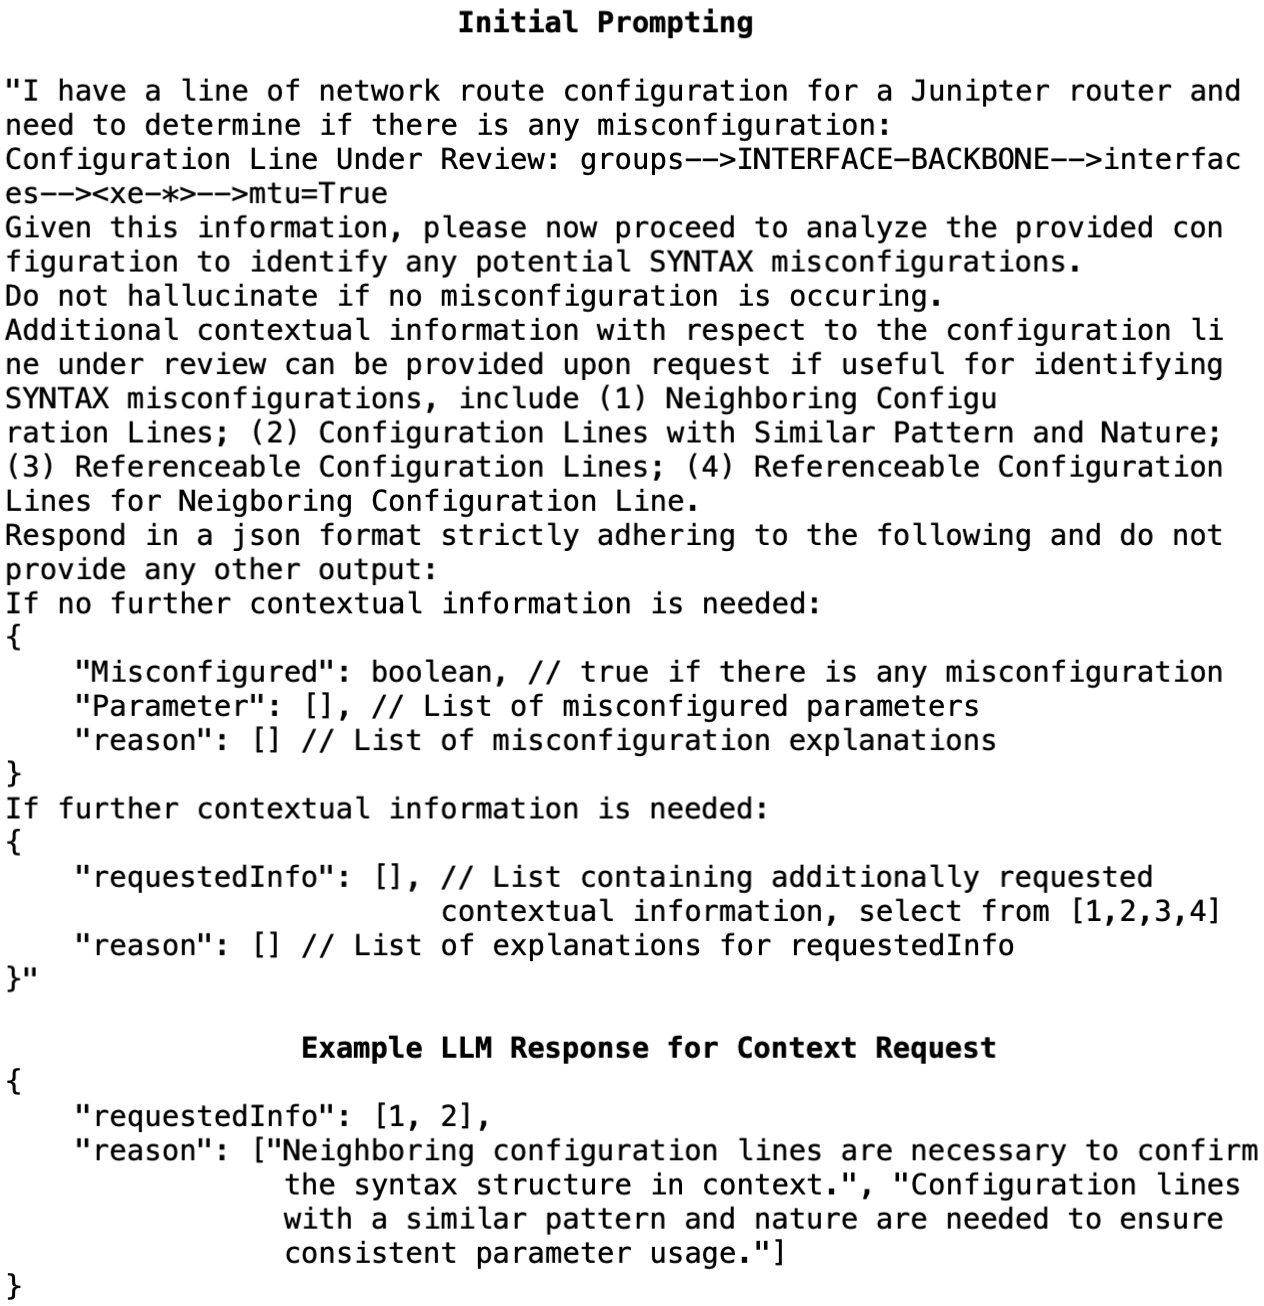
\includegraphics[width=\columnwidth]{figs/initial_prompt_response.png}}
    \caption{Example: initial prompting and LLM context request response for detecting syntax misconfiguration.}
    \label{fig:initial_prompt}
\end{figure}

    \item \textit{Contextual Options}: Next, \sysname{} offers the model the option to request additional context based on its understanding of the configuration line and the misconfiguration detection request. These options are formulated based on our categorized relevant context types, including: neighboring (\( N(P) \)), similar (\(S(P) \)) , and referenceable contexts (\( R(P) \)), as well as referenceable contexts on neighboring configurations (\( N(R(P)) \)). By allowing the model to choose which context to receive, \sysname{} ensures that the LLM is only given information that is most relevant to the detection task at hand, reducing the risk of context overload. An example request response is shown in Figure~\ref{fig:initial_prompt}.
    
    \item \textit{Iterative Refinement}: After the model processes the initial prompt, it can request additional information if needed before arriving at the final decision. \sysname{} engages in a feedback loop where the model’s output informs the next set of prompts. For instance, if the model identifies a possible syntax issue but requires more context from a related policy definition, \ie, similar context, \sysname{} can deliver that specific context in the next prompt. This iterative process continues until the model has sufficient information to make a well-informed decision. Figure~\ref{fig:feedback_and_response} provides an example of what a final misconfiguration decision looks like.
    \begin{figure}[t]
    \centering
    \fbox{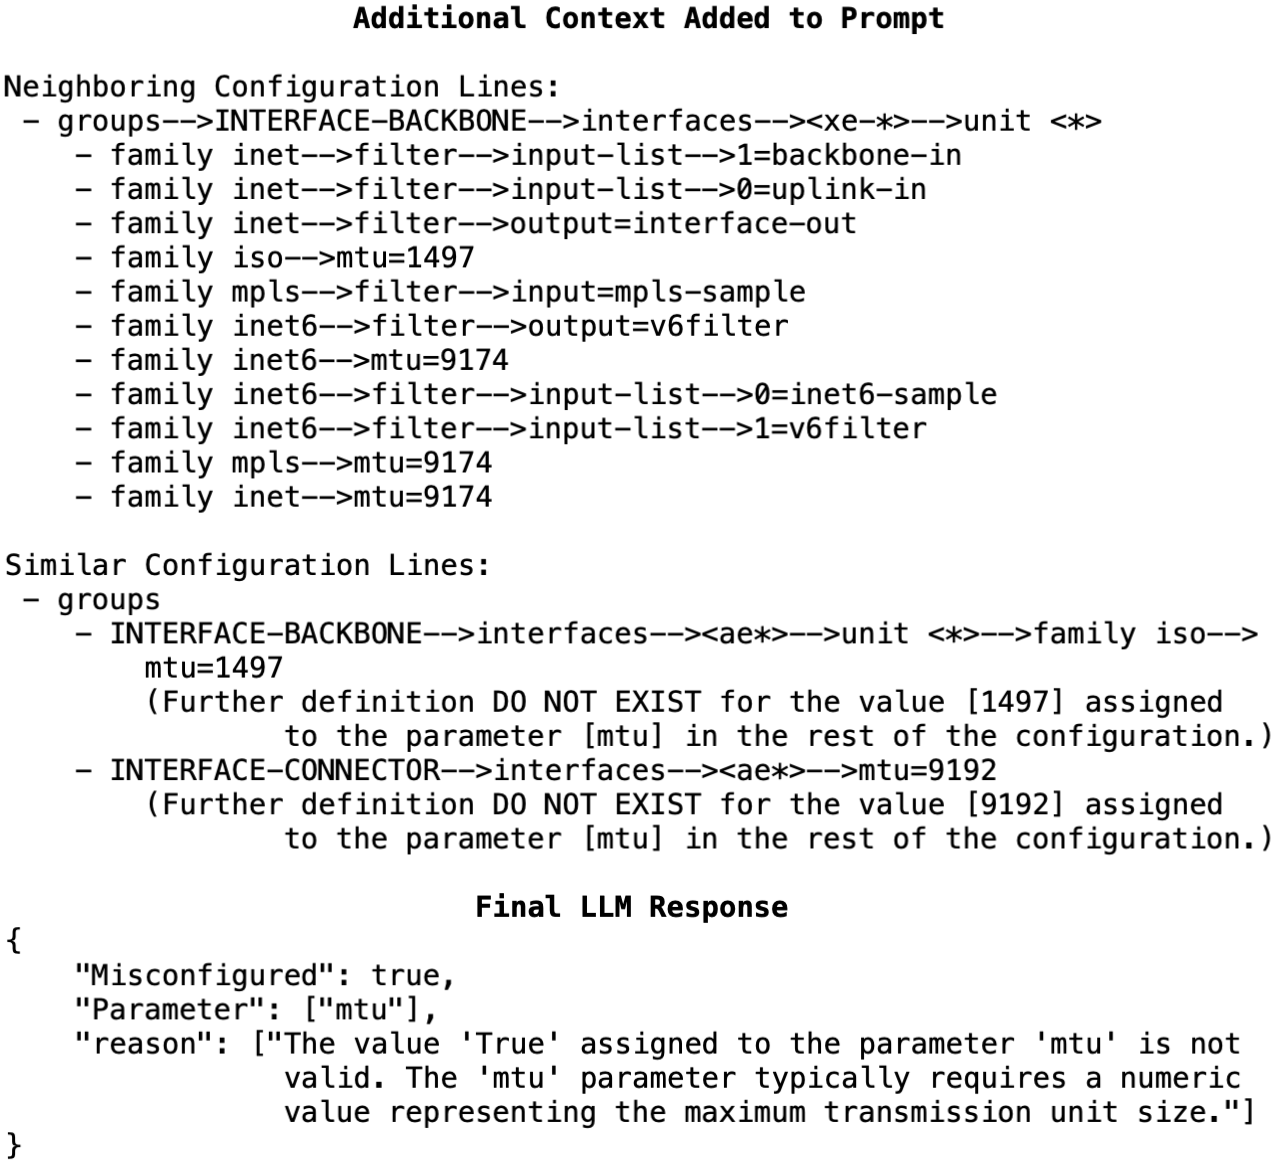
\includegraphics[width=\columnwidth]{figs/feedback_and_response.png}}
    \caption{Example: Adding requested context and retrieving misconfiguration detection result.}
    \label{fig:feedback_and_response}
\end{figure}

\end{enumerate}

This sequential, interactive approach mirrors how a network administrator might manually review a configuration file—examining the most relevant sections first, then digging deeper into referenceable or adjacent configurations as needed. It ensures that the model focuses on the most critical aspects of the configuration without becoming overwhelmed by extraneous information.

\subsubsection{Why Iterative Prompting Works}
By breaking down the context into smaller, more digestible portions, \sysname{} addresses the fundamental challenges of context overload. This method significantly enhances the model’s ability to:
\begin{enumerate}
    \item Stay on target: With less irrelevant information, the model can maintain focus on the specific configuration issue under review.
    \item Preserve coherence: Incrementally providing information allows the model to build a more coherent understanding of the configuration~\cite{li2023prompt,subramonyam2024bridging}, leading to more accurate detection of issues such as dependency conflicts or misapplied policies.
    \item Optimize performance: Avoiding context overload reduces the processing burden on the model, leading to faster and more reliable outputs.
\end{enumerate}

For example, in detecting misconfigurations in a multi-layer firewall policy, \sysname{} might first present the core rule in question, then iteratively offer neighboring rules that affect the same traffic flow, followed by referenceable configuration sections that define broader network policies. This structured process ensures that the LLM has all the information it needs, without drowning in unnecessary details, enabling it to make accurate decisions.

By combining efficient context extraction with iterative, focused interaction, \sysname{} represents a significant advancement in leveraging LLMs for router misconfiguration detection, ensuring that models are both effective and computationally efficient.